


\subsection{SYGMA: Implementation details}

The following section needs to be reworked and hence
has to be treated with care!
It is not of relevance for the user.

The program details are explained in the following while
a flow chart of the running program is given in Figure \ref{chart}.

%The main program is the chem class containing different
%functions which are called when running/creating an instance
%or afterwards for plotting or data extraction.

First the yield table files are read in using
classes in the file read\textunderscore yields.py.
The first one is a file with a 'Nugrid yield table' structure containing
yields of isotopes in solar masses plus lifetimes. Additionally,
a table containing SN1a yield data in solar masses is read.
If this file contains metallicity-dependence yields, this dependence
is adopted. Also a table file for initial abundances is read in
(Big Bang abundances) in mass fraction.

Then the program starts calculating the timesteps.
First the metallicity is of the ISM, consisting of initial abundances,
is calculated (in case of BB abundance it is 0, function getmetallicity).
Afterwards the star formation rate is calculated (function sfr).

Then the change of the ISM affected by the SFR is determined.
Important is hereby, that a part of the ISM is locked away in stars,
while (metal rich) stellar ejecta contributes to the ISM.
The ejecta is weighted by using an IMF and it is assumed
that all masses is ejected at the end of the lifetime of a star.


A delay time distribution (DTD) as specified
in Eq. 10 in Vogelsberger et al. (2013) is implemented in order
to calculate the number of SN1a events. The advantage of this
method is that progenitor, binary fraction and IMF information
is already contained. For each timestep with star formation
(new population), the contribution of SN1a ejecta of the
new population in all following timesteps is taken into account.


%For simplicity, SN1a occur for 1\% of AGB stars between 3Msun
%and 8Msun (Pritchet et al. 2008).
The function sfrmdot does all the steps mentioned above.



\begin{figure}
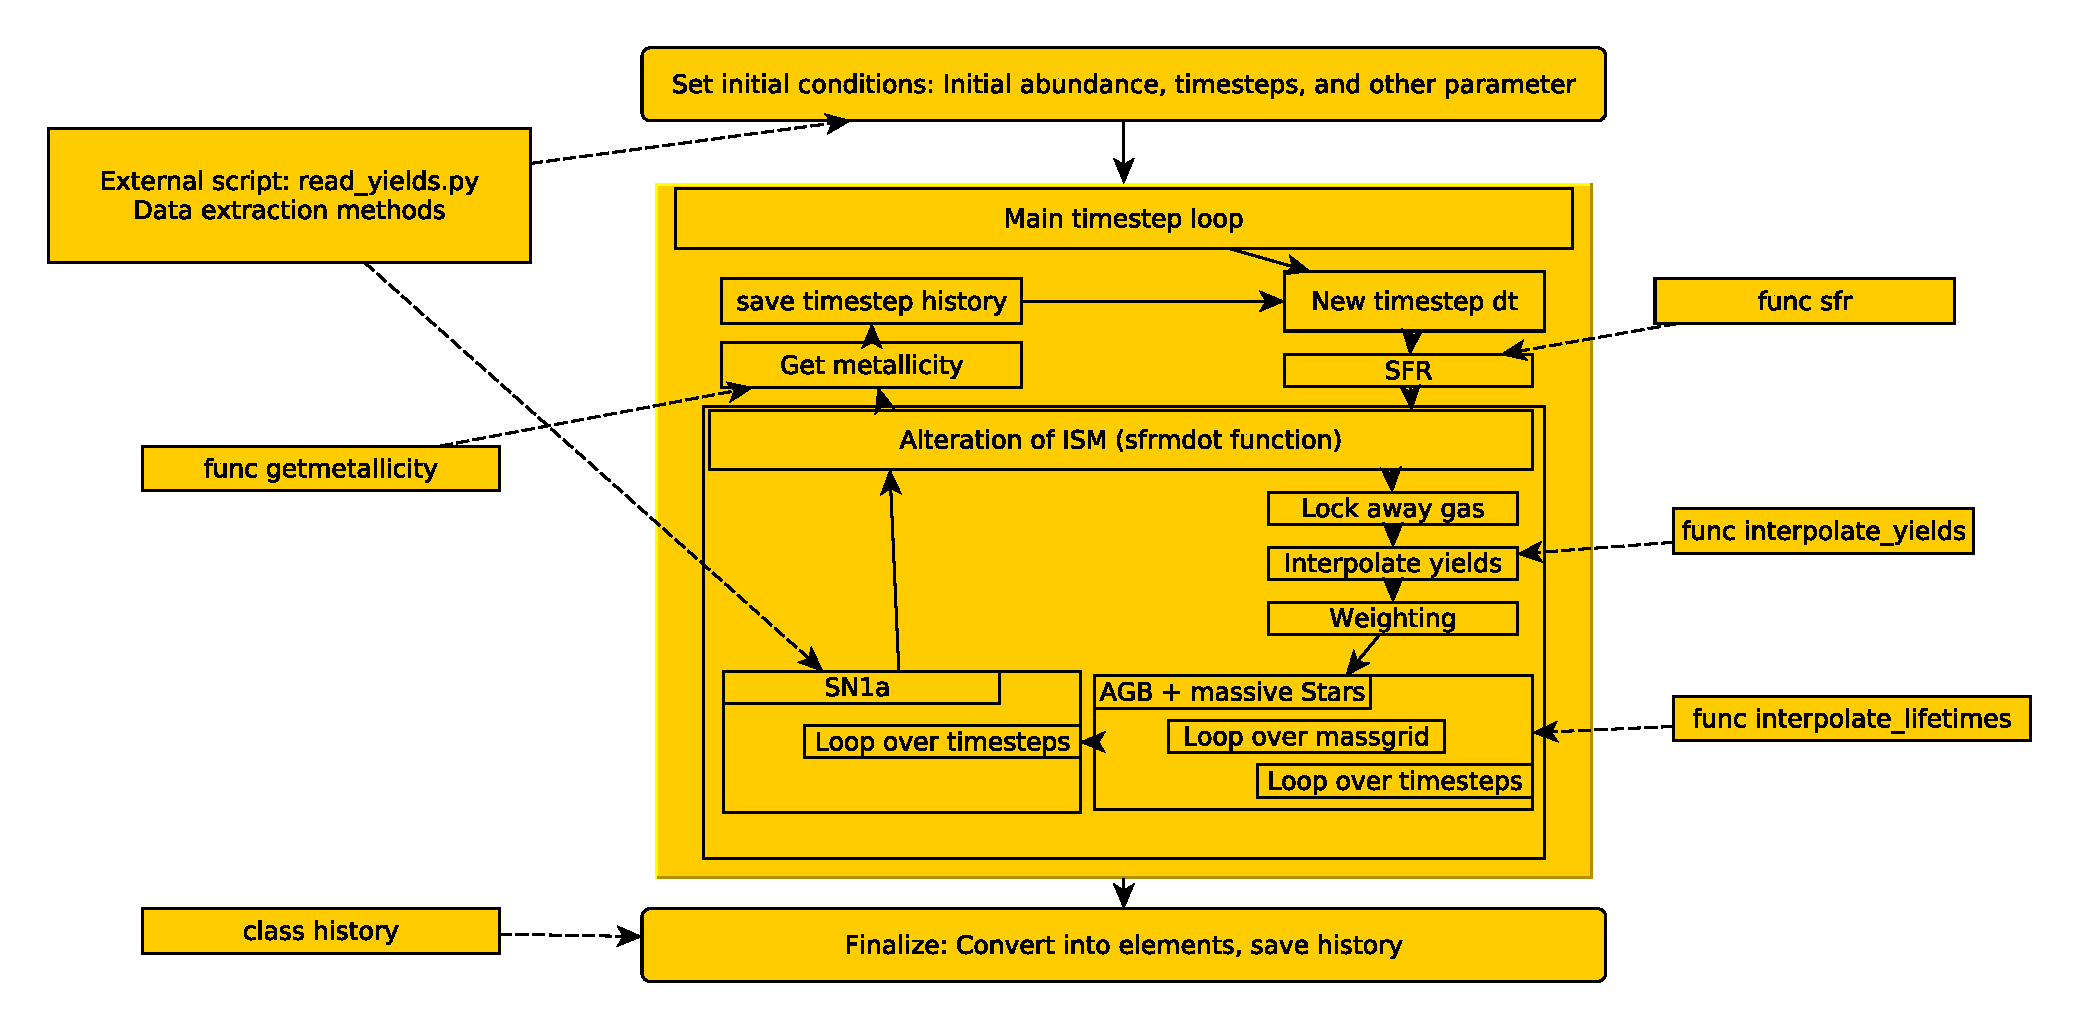
\includegraphics[width=154mm]{figures/chart.eps}
%% to include a figure, or width=84mm profile_c13_M2_1e-4
%\vspace{3.5cm}
%% to leave a blank space
\caption{Program flow}
\label{chart}
\end{figure}

\subsubsection{SN1a rate implementation}

The SN1a calculation is performed in the 
sn1a\textunderscore contribution routine (part of routine sfrmdot) which returns
the altered arrays of the ISM composition (mdot) and
SN1a\textunderscore contribution (mdot\textunderscore 1a).
There, the SN1a yield tables are read in and the proper
Z identified. In the following different implementations
are defined in subfunctions. The function vogelsberger13
describes the implementation from Vogelsberger (2013)
while the functions wiersma09\textunderscore efolding and wiersma09\textunderscore gauss
describe (the exponential and gaussian) approach used
in Wiersma (2009). For Wiersma (2009) the cumulative number
of WDs (SN1a candidates) is needed and therefore calculated
in the sfrmdot.
 
Vogelsberger: upper mass limit,8, no lower limit involved 
wiersma, mass limit:  3-8
 

Finally, for each timestep the contribution of the SN1a 
is chosen through the variable sn1a\textunderscore rate.
Also the total amount of SN1a each timestep is saved
in the array sn1a\textunderscore numbers.

In order to find the SN1a contribution of each stellar mass range to
the total ejecta the imfmass\textunderscore ranges\textunderscore contribution is calculated.
Since each mass interval is $0.1\msun$ the number of stars in
a mass range e.g. between mass $m$ and $m+0.1$ divided by the
mass range of $3$ - $8$ (which makes up the SN1a mass range contributors)
gives the fraction of the total SN1a number which came from
$m$ - $m+0.1$.


%currently hosting the implementation details, not yet to publsih

\subsubsection{Evolution of parameter with indicies}

For the reason of having an overview over the important
variables and their lengnth and indices, Fig. \ref{idxchart}
displays the GCE evolution.


\begin{figure}
\includegraphics[width=154mm]{figures/evol_index_chart.png}
%% to include a figure, or width=84mm profile_c13_M2_1e-4
%\vspace{3.5cm}
%% to leave a blank space
\caption{Evolution of parameter with indicies}
\label{idxchart}
\end{figure}


\subsubsection{Stellar lifetimes}

Recent codes (Wiersma09, Vogelsberger13)
use the  fine mass-metallicity grid of
Portinari et al. (1998) to do a interpolation
of stellar lifetimes in the mass-metallicity plane.
As mentioned by Wiersma09, lifetime depends mostly
on the mass and less on the metallicity.
In the SYGMA code, spline fits in the mass-metallicity
plane are done. First, as shown in Fig. \ref{lifetimefit}
the lifetime versus initial star mass for the grid metallicities is fitted
using spline fits. Here we use now a smoothing factor of 0 in order
to have the fit to go through all our data points (yield grid lifetimes).
(The difference for a Z=0.02 star in lifetime: 1.1770e10 (grid) vs. 1.1773e10 (fit).)
Afterwards, the fit results are used to do spline
fits over the metallicities (with same smoothing factor). This results in a '3D'-fit and
allows to retrieve necessary lifetimes for stars between
0.1 and 100Msun for different Z and initial mass.
The fitting is done in the function 
interpolate\textunderscore lifetimes.
For each mass range, corresponding to a specific yield,
the contribution of each timestep in this range is calculated.
In order to do so, a ..

\begin{figure}
\includegraphics[width=154mm]{figures/lifetime_fit.png}
%% to include a figure, or width=84mm profile_c13_M2_1e-4
%\vspace{3.5cm}
%% to leave a blank space
\caption{Fit of MS lifetime vs mass for different Z.}
\label{lifetimefit}
\end{figure}

\begin{figure}
\includegraphics[width=154mm]{figures/lifetime_fit3D.png}
%% to include a figure, or width=84mm profile_c13_M2_1e-4
%\vspace{3.5cm}
%% to leave a blank space
\caption{3D fit in the mass-metallicity plane to get the MS lifetime.}
\label{lifetimefit3D}
\end{figure}


\subsubsection{Time stepping}

The original constant-timestep implementation
(with timestep input dt) was replaced with
an exponential increasing multiplicity of
dt (in steps of dt: 1, 2, 3,...9, 10, 20, 30...100, 200...).
But between both implementations can be switched
by using the if statement in the code.



\subsubsection{The class history}

An extra class was introduced carrying
all the information about the history.
The idea is to clearly separate the 
simulation variables (needed to run
the code) and the variables saving
the results. Additionally, it is easier
to add further history variables since all
of them are at one location.

\subsubsection{Contribution sources}

In order to identify for each isotope and element
the contributing source(s) extra variables carry
the information about AGB star, SN1a and massive
star contribution. This makes the code clearly
slower, especially when calculating the elemental
contribution from the isotopic ones at the end
of the simulation.

\subsubsection{Dealing with the limited number of metallicities}

When given a certain ISM metallicity,the question arise which
models from the metallicity grid (and their yields) should be chosen.
Due to the lack of available simulations below Z=1e-4 (initial metallicity, set1.5a),
yields with initial metallicity of Z=1e-4 have to be used. In
the future Alex Heger's models might help to partly overcome this problem.
For super-solar cases the solar metallicity models are chosen.

For ISM Z values inside the grid, a interpolation of the grid yields
to the ISM metallicity has to be done.
There are different ways of interpolation. One simple way
is to linear interpolate between two metallicities of the grid 
$Z_i$, $Z_{i+1}$,
in order to get approximated yields $Y_{inter}$ at the ISM metallicity.

\begin{equation}
Y_{inter} = /(Y_i-Y_{i+1})/(Z_i-Z_{i+1}) * Z_{inter}
\end{equation}


Even though this method is used in Timmes et al. (1995)
it has clear disadvantages as explained in Wiersma et al (2009).
Another method, as motivated in the latter paper, is to split
the stellar ejecta into two components, the ones which are not
affected by the nucleosynthesis and the others which are 
produced or destroyed. As a result, a interpolation between
the ISM mass fraction and initial stellar mass fraction 
(simulation) for each isotope is done.

\begin{equation}
Eq. 6 in Wiersma et al (2009)
\end{equation}


The yield interpolation is done in the interpolate\textunderscore yields method,
in which the first, simpler method, is currently chosen.


The same assumption is used for the Z-dependent SN1a data.

\subsubsection{Choices of IMF types}

SYGMA allows to choose from the three, most popular IMF types
namely Salpeter, Chabrier and Kroupa IMF. They are chosen by
setting $imf\textunderscore type$ either to 'salpeter', 'chabrier'
or 'kroupa' respectively. In the first case the function takes
the following form

\begin{equation}
%add form with alpha here
\end{equation}

while the $\alpha$ parameter can be changed separately with
the input parameter $alphaimf$ (the default is set to 2.35).
For the Chabrier IMF, the following description is used:

\begin{equation}
%
\end{equation}

Finally, for the Kroupa IMF the form 

\begin{equation}
%
\end{equation}

is implemented.

In case a non-conventional IMF needs to be used the 
$imf\textunderscore type$ can be set to 'input' in
which case the IMF written in the file imf\textunderscore input.py is used.
\textbf{This feature needs to be more extensively tested.}



\subsubsection{IMF, mass and yield intervals}

\subsubsection{Mass intervals}

With the factor $imf$ being the GCE input one can derive for a mass interval $i$
from $m_{a,i}$ to $m_{b,i}$ the number of stars $N_i$:


\begin{equation}
N_i = k \int_{m_a}^{m_b} \Phi(m) dm
\end{equation}
where $\Phi(m)$ is the selected IMF and
$k$ being the normalization constant. 

The mass of stars in this interval can be calculated from

\begin{equation}
M_i = k \int_{m_a}^{m_b} m*\Phi(m) dm
\label{eq:imf}
\end{equation}

which allows to derive the normalization constant $k$
for a system of mass $M_{tot}$ with 

\begin{equation}
k = M_{tot} / \int_{m_a}^{m_b} m*\Phi(m) dm
\label{eq:imf}
\end{equation}

For the Salpeter IMF this results in:
\begin{equation}
N_i = k \int_{m_a}^{m_b} m^{-2.35} dm = \frac{k}{1.35} ( m_b^{-1.35} - m_a^{-1.35} ) \\
\end{equation}
\begin{equation}
k = M_{tot} /  {0.35} ( m_a^{-0.35} - m_b^{-0.35} )
\end{equation}



Due to the fact that only a limited number of simulated masses
need to covering the whole (chosen) mass range of the IMF it is necessary
to assign each mass a certain mass interval of the IMF.
The number of stars occupying each interval are then represented
by a certain simulated stellar mass and its yields.
The code calculates the number of stars in each interval as well as
the mass.

\subsubsection{Setting the total IMF range}

It is fixed in the code that only stars in the mass range between
$1\msun$ and $30\msun$ eject yields and hence have a contribution 
to the ISM.
It is possible to set the total IMF range with the parameter
$imf\textunderscore bdys$. Masses covering stars smaller than
$1\msun$ or larger than $30\msun$ are then just locked away
and not further considered.
For stars of zero metallicity ($Z=0$) a larger mass grid
of PopIII stars are available ranging from $10\msun$ to $100\msun$.


\subsubsection{Comment on SFR and input methods}

Due to the fact that this is a 1-D 'box'-model,
but star formation rates in literature are 
typically derived and given in mass per time
and per surface or volume density, the current
approach might be questionable.

In this code, the dependency of the SFR from
the area is ignored and the literature values
taken as mass per time. 

The IMF function is defined in the imf routine
which is called only in the sfrmdot routine.

\subsubsection{Extra yields sources}

In non-default mode (iniZ=-1) it is possible to
add another yields to the massive stars when
turning extra\textunderscore source\textunderscore on=True.
The code reads then another yield table provided
with the variable extra\textunderscore source\textunderscore table.
This yield table can represent for example contributions from the
r process provided by Nobuya Nishimura. (Be aware of the lower limit
of the massive star mass range).
\textbf{It might be useful to use a abundance distribution with an
extra total mass variable at some point.}

\subsection{OMEGA: Implementation details}
\label{sect_omega}
